\subsection{纤维方块投影的余均衡子}

设 X 与 Y 为拓扑空间，f 为从 X 到 Y 的一个连续映射。用 Z 表示纤维方块 \(X \times_{Y} X\)，用 \(p_{1}\) 与 \(p_{2}\) 表示从 Z 到 X 的两个投影。我们用 W 表示纤维积 \(X \times_{Y} X \times_{Y} X\)；对每个偶 \((s, t)\)（由 \(\{1,2,3\}\) 中的元素组成），用 \(q_{st}: W \to Z\) 表示由 \(q_{st}(x_{1}, x_{2}, x_{3}) = (x_{s}, x_{t})\) 定义的映射。

用 \(\operatorname{Coeg}(f)\) 表示群胚 \(\operatorname{Coeg}(\varpi(p_{1}),\varpi(p_{2}))\)，即两个态射 \(\varpi(p_{1})\)、\(\varpi(p_{2})\)（从庞加莱群胚 \(\varpi(Z)\) 到庞加莱群胚 \(\varpi(X)\)）的余均衡子。用 \(\gamma\colon\varpi(X)\to\operatorname{Coeg}(f)\) 表示规范的群胚态射。由于 \(f\circ p_{1}=f\circ p_{2}\)，群胚态射 \(\varpi(f)\circ\varpi(p_{1})\) 与 \(\varpi(f)\circ\varpi(p_{2})\)（从 \(\varpi(Z)\) 到 \(\varpi(Y)\)）相等；因此存在唯一的群胚态射 \(\varpi'(f)\colon\operatorname{Coeg}(f)\to\varpi(Y)\) 使得 \(\varpi'(f)\circ\gamma=\varpi(f)\)。

定义 1. --- 我们说映射 f 满足性质 (VK)，如果它是严格、满射的，并且态射 \(\varpi'(f)\) 是同构。

例 1. --- 在下列假设之一之下，此性质成立：

\begin{enumerate}
\def\labelenumi{(\roman{enumi})}
\item
  空间 X 与 Y 是可解圈的，空间 \(X \times_{Y} X\) 局部道路连通，映射 f 满射、逆紧、分离，且具有局部连通的纤维；
\item
  空间 X 与 Y 是可解圈的，映射 f 满射、逆紧、分离，且具有有限纤维，对角线 \(\Delta_{X}\) 在 \(X \times_{Y} X\) 中是开集且其补集局部连通；
\item
  空间 X 与 Y 是可解圈的，映射 f 满射、开，且具有道路提升性质；
\item
  Y 的每个点都有一个邻域，在该邻域之上存在映射 f 的连续截面。
\end{enumerate}

事实上，在这些假设的每一条之下，映射 \(f\) 都是满射；并且依据 I, 第~18~页，例 2，它也是严格的。最后，态射 \(\varpi'(f)\) 是同构：在假设 (i)、(ii) 或 (iii) 之下依据 IV, 第~398~页，定理 1，在假设 (iv) 之下依据（IV, 第~400~页，定理 2）。

II, 第~208~页的命题 5 描述了群胚 Coeg(f) 的迷向群。本节的目的在于：当 f 满足性质 (VK) 时，明显写出通过与群胚同构 \(\varpi'(f)\) 复合而由此得到的 Y 的庞加莱群的描述。随后的各号将用于讨论重要的特殊情形。

假设映射 f 满足性质 (VK)。

令 \(\mathsf{I} = \pi_0(\mathrm{X})\)，\(\mathsf{J} = \pi_0(\mathrm{Z})\)，\(\mathsf{K} = \pi_0(\mathrm{W})\)；对 \(j \in \mathsf{J}\) 与 \(s \in \{1,2\}\)，令 \(i_s(j) = \pi_0(p_s)(j)\)；对 \(k \in \mathsf{K}\) 与 \(s\)、\(t \in \{1,2,3\}\)，令 \(j_{st}(k) = \pi_0(q_{st})(k)\)。用 \(\Gamma\) 表示群胚态射偶 \((\varpi(p_1), \varpi(p_2))\)（从 \(\varpi(\mathrm{Z})\) 到 \(\varpi(\mathrm{X})\)）的框架（II, 第~185~页，定义 3）。它就是箭图 \((\mathsf{I}, \mathsf{J}, \pi_0(p_1), \pi_0(p_2))\)，因为拓扑空间的庞加莱群胚的轨道就是该空间的道路连通分支。

此外假设 Y 道路连通且非空。由 II, 第~200~页，注 2，\(\pi_0(\Gamma)\) 于是与群胚 Coeg(f) 的轨道集成双射；由于映射 \(f\) 满足性质 (VK)，群胚 Coeg(f) 同构于群胚 \(\varpi(Y)\)。于是图 \(\Gamma\) 连通且非空。

我们把 f 的范坎彭数据称为由下列元素组成的数据：

\begin{enumerate}
\def\labelenumi{(\roman{enumi})}
\item
  对每个 \(i \in \mathsf{I}\)，取 \(\mathsf{a}(i)\) 为道路连通分支 \(i\)（在 \(\mathbf{X}\) 中）的一点；
\item
  对每个 \(j \in J\)，取 Z 的道路连通分支 j 中的一点 \(\mathsf{b}(j) = (\mathsf{b}_{1}(j), \mathsf{b}_{2}(j))\)；
\item
  对每个 \(k \in \mathsf{K}\)，取 \(\mathsf{c}(k) = (\mathsf{c}_1(k), \mathsf{c}_2(k), \mathsf{c}_3(k))\) 为道路连通分支 \(k\)（在 \(\mathbf{W}\) 中）的一点；
\item
  对每个 \(j \in J\)，取 X 中一条道路的类 \(\beta_{1}(j)\)，该道路连接 \(\mathsf{b}_{1}(j)\) 与 \(\mathsf{a}(i_{1}(j))\)；再取 X 中一条道路的类 \(\beta_{2}(j)\)，该道路连接 \(\mathsf{b}_{2}(j)\) 与 \(\mathsf{a}(i_{2}(j))\)；
\item
  对每个 \(k \in K\) 与每个偶 \((s, t)\)（等于 \((1, 2)\)、\((2, 3)\) 或 \((1, 3)\)），取 Z 中一条道路的类 \(\gamma_{st}(k)\)，该道路连接 \((\mathsf{c}_{s}(k), \mathsf{c}_{t}(k))\) 与 \(\mathsf{b}(j_{st}(k))\)；
\item
  一个子箭图 \(\mathsf{T}\)（属于 \(\Gamma\)），其相伴图是图 \(\widetilde{\Gamma}\) 的极大树；
\item
  一个元素 \(i_{0}\)（属于 \(\mathsf{I}\)）。
\end{enumerate}

选取 \(f\) 的一个范坎彭数据。于是 \((\mathsf{a},\mathsf{b},\beta_{1},\beta_{2},\mathsf{T},i_{0})\) 是群胚态射偶 \((\varpi(p_{1}),\varpi(p_{2}))\)（从 \(\varpi(\mathrm{Z})\) 到 \(\varpi(\mathrm{X})\)）的基本配备（II, 第~192~页，定义 4）。此外，三元组

\[
\mathsf {z} = \left(\left(q _ {1 2} (\mathsf {c} (k)), 1\right), \left(q _ {2 3} (\mathsf {c} (k)), 1\right), \left(q _ {1 3} (\mathsf {c} (k)), - 1\right)\right)
\]

以及道路类 \((\gamma_{1,2}(k), \gamma_{2,3}(k), \gamma_{1,3}(k))\)（其中 k 取遍 K）定义了偶 \((\varpi(p_{1}), \varpi(p_{2}))\) 的一个补配备（II, 第~208~页，定义 3；II, 第~205~页，例；II, 第~205~页，注）。我们说如此定义的余均衡子 Coeg(f) 的完备配备是由我们所选取的 f 的范坎彭数据导出的。

对每个 \(j \in J\)，用 \(\varphi_{j} \colon \pi_{1}(Z, \mathsf{b}(j)) \to \pi_{1}(X, \mathsf{a}(i_{1}(j)))\) 与 \(\psi_{j} \colon \pi_{1}(Z, \mathsf{b}(j)) \to \pi_{1}(X, \mathsf{a}(i_{2}(j)))\) 表示由

\[
\varphi_ {j} = \operatorname{Int} (\beta_ {1} (j)) ^ {- 1} \circ (p _ {1}) _ {*}, \quad v \mapsto \beta_ {1} (j) ^ {- 1} ((p _ {1}) _ {*} (v)) \beta_ {1} (j)\tag{1}
\]

\[
\psi_ {j} = \mathrm{Int} (\beta_ {2} (j)) ^ {- 1} \circ (p _ {2}) _ {*}, \quad v \mapsto \beta_ {2} (j) ^ {- 1} ((p _ {2}) _ {*} (v)) \beta_ {2} (j),
\]

所定义的群同态，其中 \(v \in \pi_1(\mathbf{Z}, \mathfrak{b}(j))\)。对所有 \(k \in \mathsf{K}\) 与每个 \(s \in \{1,2,3\}\)，用 \(\lambda_s(k)\) 表示 X 中点 \(\mathfrak{a}(i_s(k))\) 处由下列式子定义的圈的类

\[
\lambda_ {1} (k) = \beta_ {1} (j _ {1 3} (k)) ^ {- 1} \cdot ((p _ {1}) _ {*} (\gamma_ {1 3} (k))) ^ {- 1} \cdot ((p _ {1}) _ {*} (\gamma_ {1 2} (k))) \cdot \beta_ {1} (j _ {1 2} (k)),\tag{2}
\]

\[
\lambda_ {2} (k) = \beta_ {2} (j _ {1 2} (k)) ^ {- 1} \cdot ((p _ {2}) _ {*} (\gamma_ {1 2} (k))) ^ {- 1} \cdot ((p _ {1}) _ {*} (\gamma_ {2 3} (k))) \cdot \beta_ {1} (j _ {2 3} (k)),
\]

\[
\lambda_ {3} (k) = \beta_ {2} (j _ {2 3} (k)) ^ {- 1} \cdot ((p _ {2}) _ {*} (\gamma_ {2 3} (k))) ^ {- 1} \cdot ((p _ {2}) _ {*} (\gamma_ {1 3} (k))) \cdot \beta_ {2} (j _ {1 3} (k)).
\]

用 \(\tau\) 表示从 Grp \((\Gamma)\) 到 \(\varpi(\mathrm{Y})\) 的唯一群胚态射，使得映射 Som \((\tau)\) 把 \(i \in \mathsf{I}\) 映为 \(f(\mathsf{a}(i))\)，且 Fl \((\tau)\) 把 \(j \in \mathsf{J}\) 映为道路 \(f_{*}(\beta_{1}(j))^{-1}f_{*}(\beta_{2}(j))\) 的类，该道路连接 \(f(\mathsf{a}(i_{1}(j)))\)

\pandocbounded{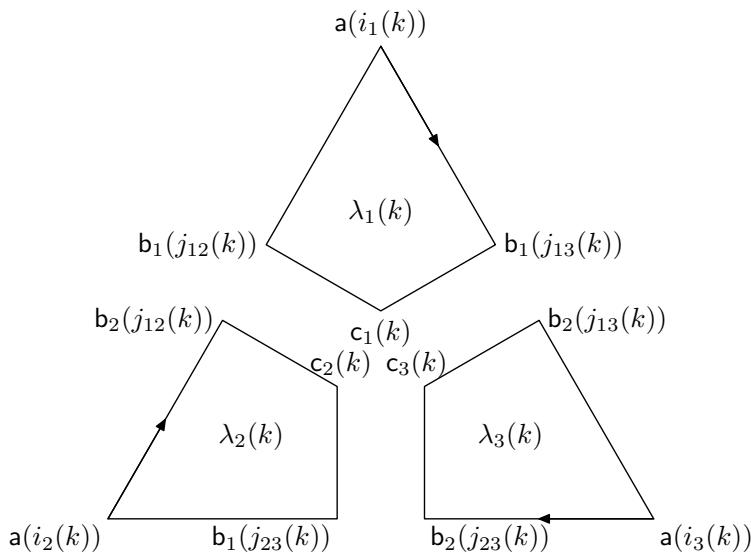
\includegraphics[keepaspectratio]{images/part003_b82e0de6.jpg}}

与 \(f(\mathsf{a}(i_2(j)))\)（在 Y 中）。对 \(i \in \mathsf{I}\)，令 \(d_i \in \mathrm{Grp}(\Gamma)\) 为连接 \(i_0\) 与 \(i\) 的唯一无折返道路（在树 \(\widetilde{\mathsf{T}}\) 中）的类，并令 \(\delta_i = \tau(d_i)\)。

回顾：若 S 是一个集合，则 F(S) 表示 S 上的自由群；在规范映射下元素 \(s \in S\) 在 F(S) 中的像记作 {[}s{]}，在不致混淆时甚至记作 s。

定理 1. --- 假设 Y 道路连通且 f 满足性质 (VK)。沿用前面的记号，存在唯一的群同态

\[
\mathsf {L} \colon \big (\underset {i \in \mathsf {I}} {\ast} \pi_ {1} (\mathrm{X}, \mathsf {a} (i)) \big) \ast \mathrm{F} (\mathrm{J}) \to \pi_ {1} (\mathrm{Y}, f (\mathsf {a} (i _ {0})))
\]

使得

\[
\begin{array}{l l} \mathsf {L} (v) = \delta_ {i} f _ {*} (v) \delta_ {i} ^ {- 1} & \text {for } i\in I \text { and } v\in\pi_{1} (X,a(i)), \\ \mathsf {L} (j) = \delta_ {i _ {1} (j)} \tau (j) \delta_ {i _ {2} (j)} ^ {- 1} & \text {for } j\in J. \end{array}
\]

此外，同态 L 是满射的，其核是包含下列元素的最小正规子群：

\[
\left(\mathrm{R} _ {1}\right) \quad \mathrm{r} _ {1} (j) = j \quad \text {for } j \text { in } \operatorname{Fl} (\mathsf {T});
\]

\[
\left(\mathrm{R} _ {2}\right) \quad \mathfrak {r} _ {2} (j, v) = \varphi_ {j} (v) j \psi_ {j} (v) ^ {- 1} j ^ {- 1} \quad \text {for } j \in \mathsf {J} \text { and } v \in \pi_ {1} (\mathrm{Z}, \mathfrak {b} (j));
\]

\[
\left(\mathrm{R} _ {3}\right) \quad \mathrm{r} _ {3} (k) = \lambda_ {1} (k) j _ {1 2} (k) \lambda_ {2} (k) j _ {2 3} (k) \lambda_ {3} (k) j _ {1 3} (k) ^ {- 1}, \quad \text {for } k \in \mathsf {K}.
\]

同态 L 的存在性与唯一性由自由积与自由群的泛性质得出。此外，这个同态是同态 \(\varpi'(f)_{\gamma(\mathsf{a}(i_0))}\)（由 \(\varpi'(f)\) 通过过渡到迷向群导出）与由 II, 第~208~页命题 5 所定义的群同态 \(\lambda\) 的复合，这里注意到所选取的范坎彭数据确定了群胚态射偶 \((\varpi(p_1), \varpi(p_2))\)（从 \(\varpi(\mathrm{Z})\) 到 \(\varpi(\mathrm{X})\)）的一个完备配备。由该命题，同态 \(\lambda\) 的像是群 \(\operatorname{Coeg}(f)_{\gamma(\mathsf{a}(i_0))}\)，其核是包含由关系 \((\mathrm{R}_1)\)、\((\mathrm{R}_2)\) 与 \((\mathrm{R}_3)\) 所定义的元素的最小正规子群。另一方面，由性质 (VK) 的定义，群胚态射 \(\varpi'(f)\) ： \(\operatorname{Coeg}(f) \to \varpi(\mathrm{Y})\) 是同构。定理于是得证。

\subsection{覆盖}

设 Y 是道路连通、非空的拓扑空间，\((\mathrm{A}_{i})_{i\in\mathrm{I}}\) 是 Y 由非空道路连通子集组成的一个覆盖，以全序集 I 为指标集。令 \(X=\bigsqcup_{i\in I}A_{i}\) 为族 \((\mathrm{A}_{i})\) 的和空间，\(f:X\to Y\) 为由每个 \(A_{i}\) 到 Y 的规范单射组成的族所诱导的映射。假设映射 f 满足性质 (VK)。特别地，这在下列两种情形成立：

\begin{enumerate}
\def\labelenumi{(\roman{enumi})}
\item
  诸集合 \(A_{i}\)（\(i \in I\)）的内部覆盖 Y（参见 IV, 第~402~页，例 2）；
\item
  空间 Y 是可解圈的，诸空间 \(A_{i}\)（\(i \in I\)）亦然，族 \((\mathrm{A}_{i})_{i \in \mathrm{I}}\) 局部有限，诸 \(A_{i}\) 在 Y 中闭，且它们两两的交局部道路连通（参见 IV, 第~399~页，例 1）。
\end{enumerate}

令 J' 为由三元组 \((i, i', V)\) 组成的集合，其中 i 与 \(i'\) 是 I 的元素，V 是 \(A_i \cap A_{i'}\) 的一个道路连通分支。若 \(j = (i, i', V) \in J'\)，则令 \(i_1(j) = i\)，\(i_2(j) = i'\)，并令 \(\overline{j} = (i', i, V)\)。令 J 为 J' 中由满足 \(i < i'\) 的三元组组成的子集。我们称覆盖的框架为这样的箭图 \(\Gamma\)：其顶点集为 I，箭集为 J，源映射与靶映射分别为映射 \(j \mapsto i_1(j)\) 与 \(j \mapsto i_2(j)\)。我们将把与 \(\Gamma\) 相伴的图等同于这样的图 \(\widetilde{\Gamma}\)：其顶点集为 I，箭集为 \(J \cup \overline{J}\)，源映射与靶映射为映射 \(j \mapsto i_{1}(j)\) 与 \(j \mapsto i_{2}(j)\)，其对合为映射 \(j \mapsto \overline{j}\)。

用 \(p_1\) 与 \(p_2\) 表示纤维方块 \(X \times_{Y} X\) 到 X 上的投影；令 \(\textsf{Γ}\) 为群胚态射偶 \((\varpi(p_1), \varpi(p_2))\)（从 \(\varpi(\mathrm{X} \times_{\mathrm{Y}} \mathrm{X})\) 到 \(\varpi(\mathrm{X})\)）的框架。

引理 1. --- 箭图 \(\Gamma\) 可等同于 \(\textsf{Γ}\) 的一个子箭图；箭图 \(\Gamma\) 与 \(\textsf{Γ}\) 都是连通的。

X 的道路连通分支是诸 \(A_{i}\)（\(i \in I\)）。\(X \times_{Y} X\) 的道路连通分支是诸 \((V \times \{i\}) \times_{Y} (V \times \{i'\})\)（\((i, i', V) \in J'\)）。于是，框架 \(\textsf{Γ}\)（属于偶 \((\varpi(p_1), \varpi(p_2))\)）同构于这样的箭图：其顶点集为 I，箭集为 \(J'\)，源映射与靶映射分别为映射 \(j \mapsto i_1(j)\) 与 \(j \mapsto i_2(j)\)。箭图 \(\textsf{Γ}\) 是连通的（IV, 第~406~页）。此外，这一描述把 \(\Gamma\) 等同于 \(\textsf{Γ}\) 的一个子箭图。我们还注意到，对 \(\textsf{Γ}\) 的每条箭 j，或者 \(j \in \mathrm{Fl}(\widetilde{\Gamma})\)，或者存在 \(i \in I\) 使得 \(j = (i, i, A_i)\)。由此推出，映射 \(\pi_0(\Gamma) \to \pi_0(\textsf{Γ})\)（由 \(\Gamma\) 到 \(\textsf{Γ}\) 的单射导出）是双射，从而 \(\textsf{Γ}\) 是连通的。

对 I 的每个元素 \(i\)，选取一点 \(a(i)\)（在 \(\mathrm{A}_i\) 中）。

对每个元素 \(j = (i, i', \mathrm{V})\)（属于 \(\mathrm{J}\)），选取一点 \(b(j)\)（在 \(\mathrm{V}\) 上）、一条道路 \(\mathrm{B}_1(j)\)，它连接 \(b(j)\) 与 \(a(i)\)（在 \(\mathrm{A}_i\) 上），以及一条道路 \(\mathrm{B}_2(j)\)，它连接 \(b(j)\) 与 \(a(i')\)（在 \(\mathrm{A}_{i'}\) 上）。设 \(j = (i, i', \mathrm{V})\) 是 \(\overline{\mathrm{J}}\) 的一个元素；则 \(\overline{j} = (i', i, \mathrm{V})\) 属于 \(\mathrm{J}\)，且令 \(b(\overline{j}) = b(j)\)，\(\mathrm{B}_1(j) = \mathrm{B}_2(\overline{j})\)，\(\mathrm{B}_2(j) = \mathrm{B}_1(\overline{j})\)。对 \(j \in \mathrm{J}' \cup \overline{\mathrm{J}'}\)，道路 \(\overline{\mathrm{B}_1(j)}\) 与 \(\mathrm{B}_2(j)\)（在 \(\mathrm{Y}\) 上）是可拼接的。令

\[
\mathrm{B} (j) = \overline {{\mathrm{B} _ {1} (j)}} * \mathrm{B} _ {2} (j).\tag{3}
\]

这是 Y 中连接 \(a(i_1(j))\) 与 \(a(i_2(j))\) 的一条道路；我们有关系式 \(\mathrm{B}(\overline{j}) = \overline{\mathrm{B}(j)}\)。

对每个 \(j = (i, i', \mathrm{V}) \in \mathrm{J}'\)，用 \(p_{j,1} \colon V \to A_i\) 与 \(p_{j,2} \colon V \to A_{i'}\) 表示规范单射；再用 \(\varphi_j \colon \pi_1(\mathrm{V}, b(j)) \to \pi_1(\mathrm{A}_i, a(i))\) 与 \(\psi_j \colon \pi_1(\mathrm{V}, b(j)) \to \pi_1(\mathrm{A}_{i'}, a(i'))\) 表示由

\[
\varphi_ {j} (v) = [ \mathrm{B} _ {1} (j) ] ^ {- 1} (p _ {j, 1}) _ {*} (v) [ \mathrm{B} _ {1} (j) ]
\]

以及

\[
\psi_ {j} (v) = [ \mathrm{B} _ {2} (j) ] ^ {- 1} (p _ {j, 2}) _ {*} (v) [ \mathrm{B} _ {2} (j) ],
\]

所定义的群同态，其中 \(v \in \pi_1(\mathrm{V}, b(j))\)（参见 IV, 第~407~页）。

固定 I 的一个元素 \(i_0\)，以及箭图 \(\Gamma\) 中的一个子箭图 T，其相伴图 \(\widetilde{T}\) 是图 \(\widetilde{\Gamma}\) 的极大树。

对 \(i \in I\)，设 \((i_0, j_1, i_1, \ldots, j_n, i)\) 是连接 \(i_0\) 与 \(i\) 的唯一无折返道路（在树 \(\widetilde{T}\) 中），并令

\[
\delta (i) = \left[ \mathrm{B} \left(j _ {1}\right) \right] \left[ \mathrm{B} \left(j _ {2}\right) \right] \dots \left[ \mathrm{B} \left(j _ {n}\right) \right];
\]

它是 Y 中连接 \(a(i_0)\) 与 \(a(i)\) 的一条道路的类。用 \(\alpha_i\) 表示由规范单射导出的从 \(\pi_1(\mathrm{A}_i, a(i))\) 到 \(\pi_1(\mathrm{Y}, a(i))\) 的同态，并令 \(\mu_i: \pi_1(\mathrm{A}_i, a(i)) \to \pi_1(\mathrm{Y}, a(i_0))\) 为由下式定义的群同态：

\[
\mu_ {i} (v) = \delta (i) \alpha_ {i} (v) \delta (i) ^ {- 1}.
\]

最后，令 \(\mu\colon\mathrm{F}(\mathrm{J})\to\pi_{1}(\mathrm{Y},a(i_{0}))\) 为唯一的群同态，使得

\[
\mu (j) = \delta (i _ {1} (j)) [ \mathrm{B} (j) ] \delta (i _ {2} (j)) ^ {- 1}
\]

对所有 \(j \in J\) 成立。存在唯一的群同态

\[
\mathsf {M} \colon \big (\underset {i \in \mathrm{I}} {\ast} \pi_ {1} (\mathrm{A} _ {i}, a (i)) \big) \ast \mathrm{F} (\mathrm{J}) \to \pi_ {1} (\mathrm{Y}, a (i _ {0}))
\]

它与 \(\mu_i\) 在每个 \(\pi_1(A_i, a(i))\)（\(i \in I\)）上、与 \(\mu\) 在 \(F(J)\) 上一致。

令 K' 为由四元组 \((i_{1}, i_{2}, i_{3}, \mathrm{U})\) 组成的集合，其中 \(i_{1}, i_{2}, i_{3}\) 是 I 的元素，U 是 \(A_{i_{1}} \cap A_{i_{2}} \cap A_{i_{3}}\) 的一个道路连通分支。对每个元素 \(k = (i_{1}, i_{2}, i_{3}, \mathrm{U})\)（属于 \(K'\)）与每个偶 \((s, t)\)（由 \(\{1, 2, 3\}\) 中的元素组成），令 \(j_{st}(k) = (i_{s}, i_{t}, \mathrm{V})\)，其中 V 是包含 U 的 \(A_{i_{s}} \cap A_{i_{t}}\) 的道路连通分支；这是 \(J'\) 的一个元素。

令 K 为 \(K'\) 中由四元组 \((i_{1}, i_{2}, i_{3}, \mathrm{U})\)（满足 \(i_{1} < i_{2} < i_{3}\)）组成的子集。对 K 的每个元素 \(k = (i_{1}, i_{2}, i_{3}, \mathrm{U})\)，选取 U 的一点 \(c(k)\)，以及道路 \(\mathrm{C}_{12}(k)\)、\(\mathrm{C}_{23}(k)\) 与 \(\mathrm{C}_{13}(k)\)，使得 \(\mathrm{C}_{st}(k)\) 连接 \(c(k)\) 与 \(b(j_{st}(k))\)（在 \(A_{i_{s}} \cap A_{i_{t}}\) 中），这里 \(s, t \in \{1, 2, 3\}\) 满足 s \textless{} t。

然后，对 \(k \in \mathbf{K}\)，令

\[
\mathrm{L} _ {1} (k) = \overline {{\mathrm{B} _ {1} (j _ {1 3} (k))}} * \overline {{\mathrm{C} _ {1 3} (k)}} * \mathrm{C} _ {1 2} (k) * \mathrm{B} _ {1} (j _ {1 2} (k)),\tag{4}
\]

\[
\mathrm{L} _ {2} (k) = \overline {{\mathrm{B} _ {2} (j _ {1 2} (k))}} * \overline {{\mathrm{C} _ {1 2} (k)}} * \mathrm{C} _ {2 3} (k) * \mathrm{B} _ {1} (j _ {2 3} (k)),
\]

\[
\mathrm{L} _ {3} (k) = \overline {{\mathrm{B} _ {2} (j _ {2 3} (k))}} * \overline {{\mathrm{C} _ {2 3} (k)}} * \mathrm{C} _ {1 3} (k) * \mathrm{B} _ {2} (j _ {1 3} (k)).
\]

对 \(s \in \{1,2,3\}\)，用 \(\lambda_s(k)\) 表示 \(\pi_1(\mathrm{A}_{i_s}, a(i_s))\) 中圈 \(\mathrm{L}_s(k)\) 的类。

命题 1. --- 设 Y 是道路连通的拓扑空间，\((\mathrm{A}_{i})_{i\in\mathrm{I}}\) 是 Y 由非空道路连通子集组成、以全序集 I 为指标集的一个覆盖。假设族 \((\mathrm{A}_{i})_{i\in\mathrm{I}}\) 的和空间到 Y 中的规范映射满足性质 (VK)。那么，上面引入的同态 M 是满射的，其核是包含下列元素的最小正规子群：

\[
\begin{array}{l} \text {(R$_ {1}$)} r _ {1} (j) = j \qquad \text {for } j \text { in } \operatorname{Fl}(\mathsf {T}); \\ \text {(R$_ {2}$)} r _ {2} (j, v) = \varphi_ {j} (v) j \psi_ {j} (v) ^ {- 1} j ^ {- 1} \\ \qquad \qquad \qquad \qquad \qquad \qquad \qquad \qquad \qquad \text {for } j = (i,i^{\prime} ,V)\in \mathsf {J} \text { and } v\in\pi_{1} (V,b(j)); \\ \text {(R$_ {3}$)} r _ {3} (k) = \lambda_ {1} (k) j _ {1 2} (k) \lambda_ {2} (k) j _ {2 3} (k) \lambda_ {3} (k) j _ {1 3} (k) ^ {- 1} \\ \qquad \qquad \qquad \qquad \qquad \qquad \qquad \qquad \text {for } k\in \mathsf {K}. \end{array}
\]

设 X 是族 \((\mathrm{A}_{i})_{i\in\mathrm{I}}\) 的和所成的拓扑空间，\(f\colon X\to Y\) 为由每个 \(A_{i}\) 到 Y 的规范单射组成的族所诱导的映射。由假设，映射 f 满足性质 (VK)；因此我们将对它应用第 1 号的定理 1。于是我们沿用该节的记号，并从为映射 f 定义一个范坎彭数据开始。

X 的道路连通分支是诸集合 \(X_{i} = A_{i} \times \{i\}\)（\(i \in I\)）。这样就把 \(\pi_{0}(X)\) 等同于集合 I。对每个 \(i \in I\)，用 \(\mathfrak{a}(i)\) 表示点 \((a(i), i)\)（属于 \(X_{i}\)）。

令 \(Z = X \times_{Y} X\)。\(Z\) 的道路连通分支是诸集合 \(Z_j = (V \times \{i\}) \times_{Y} (V \times \{i'\})\)，其中 \(j = (i, i', V)\) 取遍 \(J'\)。这样就把 \(\pi_0(Z)\) 等同于集合 \(J'\)。令 \(J_0\) 为 \(J\) 中形如 \((i, i, A_i)\) 的元素组成的集合，于是族 \((J_0, J, \overline{J})\) 是 \(J'\) 的一个划分。对 \(i \in I\) 与 \(j = (i, i, A_i) \in J_0\)，令 \(b(j) = (a(i), a(i))\)，并取 \(\beta_1(j)\) 与 \(\beta_2(j)\) 为 \(a(i)\) 处常值道路的类。对 \(j = (i, i', V) \in J \cup \overline{J}\)，用 \(b(j)\) 表示点 \(((b(j), i), (b(j), i'))\)（属于 \(Z_j\)），并用 \(\beta_1(j)\) 与 \(\beta_2(j)\) 表示道路 \(t \mapsto (B_1(j)(t), i)\) 与 \(t \mapsto (B_2(j)(t), i')\)（在 \(X\) 上）的类。

令 \(W = X \times_{Y} X \times_{Y} X\)。W 的道路连通分支是诸集合 \(W_k = (U \times \{i_1\}) \times_{Y} (U \times \{i_2\}) \times_{Y} (U \times \{i_3\})\)，其中 \(k = (i_1, i_2, i_3, U)\) 取遍 \(K'\)。这样就把 \(\pi_0(W)\) 等同于集合 \(K'\)。

用 \(K_{0}\) 表示 \(K'\) 中形如 \(k = (i, i, i, A_{i})\)（\(i \in I\)）的元素组成的集合。对这样的元素 \(k \in K_{0}\)，令 \(\mathsf{c}(k) = (\mathsf{a}(i), \mathsf{a}(i), \mathsf{a}(i))\)，并取 \(\gamma_{st}(k)\) 为 \((\mathsf{a}(i), \mathsf{a}(i))\) 处常值道路的类。

用 \(K_{1}\) 表示 \(K'\) 中形如 \(k = (i_{1}, i_{2}, i_{3}, V)\) 且集合 \(\{i_{1}, i_{2}, i_{3}\}\) 恰有两个元素的元素组成的集合。设 k 是 \(K'\) 中形如 \((i, i, i', V)\) 的元素，使得 \(j = (i, i', V)\) 属于 \(J \cup \overline{J}\)。这时令

\[
\mathsf {c} (k) = ((b (j), i), (b (j), i), (b (j), i ^ {\prime})), \quad \gamma_ {1 2} (k) = (\beta_ {1} (j), \beta_ {1} (j))
\]

并取 \(\gamma_{13}(k)\) 与 \(\gamma_{23}(k)\) 为 \(\mathsf{b}(j)\) 处常值道路的类。类似地定义 \(c(k)\)、\(\gamma_{12}(k)\)、\(\gamma_{13}(k)\)、\(\gamma_{23}(k)\)（对每个元素 \(k\)，属于 \(\mathrm{K}'\)）。

对 K 的每个元素 \(k = (i_{1}, i_{2}, i_{3}, \mathrm{U})\)，令

\[
\mathsf {c} (k) = ((c (k), i _ {1}), (c (k), i _ {2}), (c (k), i _ {3})) ;
\]

对每个偶 \((s,t)\)（由 \(\{1,2,3\}\) 中不同元素组成），取 \(\gamma_{st}(k)\) 为映射 \(x\mapsto((x,s),(x,t))\) 对道路 \(\mathrm{C}_{st}(k)\) 在 \(\mathrm{A}_{i_{s}(k)}\cap\mathrm{A}_{i_{t}(k)}\) 中的类所取的像。

对每个点 \(x = (x_1, x_2, x_3)\)（属于 \(X \times_Y X \times_Y X\)）与每个置换 \(\sigma \in \mathfrak{S}_3\)，令 \(\sigma(x) = (x_{\sigma^{-1}(1)}, x_{\sigma^{-1}(2)}, x_{\sigma^{-1}(3)})\)。这样就定义了群 \(\mathfrak{S}_3\) 在 W 上的一个作用。对每个 \(k = (i_1, i_2, i_3, U) \in K'\) 与每个置换 \(\sigma \in \mathfrak{S}_3\)，类似地令 \(\sigma(k) = (i_{\sigma^{-1}(1)}, i_{\sigma^{-1}(2)}, i_{\sigma^{-1}(3)}, U)\)；我们有

\[
\sigma \left(\mathrm{W} _ {k}\right) = \left(\mathrm{U} \times \left\{i _ {\sigma^ {- 1} (1)} \right\}\right) \times_ {\mathrm{Y}} \left(\mathrm{U} \times \left\{i _ {\sigma^ {- 1} (2)} \right\}\right) \times_ {\mathrm{Y}} \left(\mathrm{U} \times \left\{i _ {\sigma^ {- 1} (3)} \right\}\right) = \mathrm{W} _ {\sigma (k)}.
\]

设 \(k = (i_1, i_2, i_3, \mathrm{U})\) 是 \(\mathrm{K}'\) 的元素，且 \(i_1, i_2, i_3\) 两两不同。存在唯一的置换 \(\sigma \in \mathfrak{S}_3\) 使得 \(i_{\sigma^{-1}(1)} < i_{\sigma^{-1}(2)} < i_{\sigma^{-1}(3)}\)，亦即使得 \(\sigma(k) = (i_{\sigma^{-1}(1)}, i_{\sigma^{-1}(2)}, i_{\sigma^{-1}(3)}, \mathrm{U})\) 属于 \(\mathrm{K}\)。对 \(s \in \{1, 2, 3\}\)，令 \(c_s(k) = c_{\sigma(s)}(\sigma(k))\)，\(c(k) = (c_1(k), c_2(k), c_3(k))\)，于是 \(c(k) = \sigma^{-1}(c(\sigma(k)))\)。对 \((s, t) \in \{(1, 2), (1, 3), (2, 3)\}\)，定义 \(\mathrm{C}_{st}(k) = \mathrm{C}_{\sigma^{-1}(s)\sigma^{-1}(t)}(\sigma(k))\)；这是连接 \(c(k)\) 与 \(b(j_{\sigma(s)\sigma(t)}(\sigma(k))) = b(j_{st}(k))\) 的一条道路。

用 \(g\) 表示从 \(\Gamma\) 到 \(\textsf{Γ}\) 的箭图态射，它把顶点 \(i \in I\)（属于 \(\Gamma\)）对应为顶点 \(X_i = A_i \times \{i\}\)（属于 \(\textsf{Γ}\)），把箭 \(j = (i, i', V) \in J'\)（属于 \(\Gamma\)）对应为箭 \(Z_j = (V \times \{i\}) \times_Y(V \times \{i'\})\)（属于 \(\textsf{Γ}\)）。映射 Som( \(g\) ) 是双射；映射 Fl( \(g\) ) 是单射，且图 \(\Gamma\) 连通（IV, 第~410~页，引理 1），并且子箭图 T 在 \(g\) 下的像是一个子箭图 \(\mathsf{T}\)（属于 \(\textsf{Γ}\)），其相伴图是图 \(\widetilde{\textsf{Γ}}\) 的极大树。

诸点 \(\mathsf{a}(i)\)（\(i \in I\)）、点 \(\mathsf{b}(j)\)（\(j \in J'\)）、诸点 \(\mathsf{c}(k)\)（\(k \in K'\)）、道路类 \(\beta_{1}(j)\) 与 \(\beta_{2}(j)\)（\(j \in J'\)）、道路类 \(\gamma_{st}(k)\)（\(k \in \mathrm{K}'\)）、子箭图 \(g(\mathrm{T})\)（属于 \(\textsf{Γ}\)）以及元素 \(i_0\)（属于 I）定义了 \(f\) 的一个范坎彭数据。

用 \(\rho\) 表示唯一的群同态

\[
\rho \colon \big (\underset {i \in \mathrm{I}} {*} \pi_ {1} (\mathrm{X}, \mathsf {a} (i)) \big) * \mathrm{F} (\mathrm{J} ^ {\prime}) \to \big (\underset {i \in \mathrm{I}} {*} \pi_ {1} (\mathrm{A} _ {i}, a (i)) \big) * \mathrm{F} (\mathrm{J})
\]

它在 \(\pi_1(\mathrm{X},\mathsf{a}(i))\) 与 \(\pi_1(\mathrm{A}_i,a(i))\) 之间诱导出由 \(\mathrm{A}_i\times \{i\}\) 与 \(\mathrm{A}_i\) 的等同所导出的同构（对每个 \(i\in \mathrm{I}\)），并且使得

\[
\begin{array}{l l} \rho (j) = 1 & \text {for } j \in \mathrm{J} _ {0} \\ \rho (j) = j, \quad \rho (\overline {{j}}) = j ^ {- 1} & \text {for } j \in \mathrm{J}. \end{array}
\]

设 L 为 IV, 第~408~页定理 1 中所定义的群同态。对 \(j = (i, i, \mathrm{A}_i) \in \mathrm{J}_0\)，我们有 \(\mathsf{L}(j) = 1 = \mathsf{M} \circ \rho(j)\)。设 \(j = (i, i', \mathrm{V})\) 是 J 的一个元素；由定义我们有 \(\mathsf{L}(j) = (\mathsf{M} \circ \rho)(j)\)。最后，若 \(j = (i, i', \mathrm{V})\) 是 \(\overline{\mathbf{J}}\) 的一个元素，则 \(\overline{j} \in \mathbf{J}\)，并且可以验证

\[
\mathsf {L} (j) = \mathsf {L} (\overline {{j}}) ^ {- 1} = \mathsf {M} (\rho (\overline {{j}})) ^ {- 1} = \mathsf {M} (\rho (j)).
\]

于是，我们有 M ∘ ρ = L。

同态 L 是满射的（出处同上），因此同态 M 也是满射的。由于同态 \(\rho\) 是满射的，M 的核是 \(\left(\ast\pi_{1}(\mathrm{A}_{i},a(i))\right)*\mathrm{F}(\mathrm{J})\) 中包含在 \(\rho\) 下定理 1（IV, 第~408~页）的关系 \((\mathrm{R}_{1})\)、\((\mathrm{R}_{2})\)、\((\mathrm{R}_{3})\) 所定义元素的像的最小正规子群。只需验证这些像，除了命题 1 的关系 \((\mathrm{R}_{1})\)、\((\mathrm{R}_{2})\)、\((\mathrm{R}_{3})\) 所定义的元素之外，还包括与它们共轭的元素、或与其逆共轭的元素，以及单位元，证明即告完成。

元素 R \(_{1}\) --- 定向树 T 的一条箭形如 Z \(_{j}\)，其中 \(j = (i, i', V) \in J\)；它的像是 F(J) 的元素 \(j\)。

元素 R₂. --- 设 \(j = (i, i', \mathrm{V}) \in \mathrm{J}'\)。若 \(i = i'\)，我们有 \(\rho(\mathsf{r}_2(j, v)) = 1\)（对所有 \(v \in \pi_1(\mathrm{A}_i, \mathsf{a}(i))\)）。若 \(j \in J\)，则 \(\mathsf{r}_2(j, v)\) 的像是元素 \(r_2(j, v) = \varphi_j(v) j \psi_j(v)^{-1} j^{-1}\)（对每个 \(v \in \pi_1(\mathrm{Z}, \mathsf{b}(j))\)）。在余下的情形，我们有 \(\overline{j} \in J\)，且等式

\[
\begin{array}{r l} & {\rho (\mathtt {r} _ {2} (j, v)) = \rho (\varphi_ {j} (v) j \psi_ {j} (v) ^ {- 1} j ^ {- 1})} \\ & {\qquad = [ \mathrm{B} _ {1} (j) ] ^ {- 1} v [ \mathrm{B} _ {1} (j) ] \rho (j) [ \mathrm{B} _ {2} (j) ] ^ {- 1} v ^ {- 1} [ \mathrm{B} _ {2} (j) ] \rho (j) ^ {- 1}} \\ & {\qquad = [ \mathrm{B} _ {2} (\bar {j}) ] ^ {- 1} v [ \mathrm{B} _ {2} (\bar {j}) ] \bar {j} ^ {- 1} [ \mathrm{B} _ {1} (\bar {j}) ] ^ {- 1} v ^ {- 1} [ \mathrm{B} _ {1} (\bar {j}) ] \bar {j}} \end{array}
\]

表明 \(\rho(\mathsf{r}_2(j,v))\) 与 \(\rho(\mathsf{r}_2(\overline{j},v^{-1}))\) 共轭。

元素 R₃. — 设 \(k = (i_{1}, i_{2}, i_{3}, \mathrm{U})\) 是 K' 的一个元素。

若 \(k \in \mathrm{K}_0\)，则 \(i_1 = i_2 = i_3\)，\(\lambda_s(k)\) 对所有 \(s \in \{1,2,3\}\) 是平凡道路的类，且 \(j_{st}(k) \in \mathrm{J}_0\) 对每个偶 \((s,t) \in \{(1,2),(1,3),(2,3)\}\) 成立。此时 \(\rho(\mathsf{r}_3(k))\) 是单位元。

设 \(k\in \mathrm{K}_1\)。若 \(i_1 = i_2\)，则 \(j = (i_{1},i_{3},\mathrm{U})\in \mathrm{J}\cup \overline{\mathrm{J}}\)，并且有

\[
\mathsf {r} _ {3} (k) = \beta_ {1} (j) ^ {- 1} j _ {1 2} \beta_ {1} (j) j _ {2 3} \beta_ {2} (j) ^ {- 1} \beta_ {2} (j) j _ {1 3} ^ {- 1}
\]

它在 \(\rho\) 下的像是单位元。其余情形类似处理。

设 \(i_{1}, i_{2}, i_{3}\) 两两不同。若 \(i_{1} < i_{2} < i_{3}\)，则 \(k \in \mathbf{K}\)，且 \(\rho(\mathsf{r}_{3}(k))\) 的像是元素 \(r_{3}(k)\)。

设 \(\sigma \in \mathfrak{S}_3\) 为把 1 映到 2、把 2 映到 3 的置换。我们有

\[
\begin{array}{r l} \lambda_ {1} (\sigma (k)) & = \beta_ {1} (j _ {1 3} (\sigma (k))) ^ {- 1} \cdot p _ {1, *} (\gamma_ {1 3} (\sigma (k))) ^ {- 1} \cdot \\ & \qquad \cdot p _ {1, *} (\gamma_ {1 2} (\sigma (k))) \cdot \beta_ {1} (j _ {1 2} (\sigma (k))) \\ & = \beta_ {1} (j _ {3 2} (k)) ^ {- 1} \cdot p _ {1, *} (\gamma_ {3 2} (k)) ^ {- 1} \cdot p _ {1, *} (\gamma_ {3 1} (k)) \cdot \beta_ {1} (j _ {3 1} (k)) \\ & = \beta_ {2} (j _ {2 3} (k)) ^ {- 1} \cdot p _ {2, *} (\gamma_ {2, 3} (k)) ^ {- 1} \cdot p _ {2, *} (\gamma_ {1 3} (k)) \cdot \beta_ {2} (j _ {1 3} (k)) \\ & = \lambda_ {3} (k). \end{array}
\]

我们类似地验证 \(\lambda_2(\sigma(k)) = \lambda_1(k)\) 与 \(\lambda_3(\sigma(k)) = \lambda_2(k)\)。于是，

\[
\begin{array}{r l} & {\rho (\mathsf {r} _ {3} (\sigma (k))) = \lambda_ {1} (\sigma (k)) \rho (j _ {1 2} (\sigma (k))) \lambda_ {2} (\sigma (k)) \cdot} \\ & {\qquad \cdot \rho (j _ {2 3} (\sigma (k))) \lambda_ {3} (\sigma (k)) \rho (j _ {1 3} (\sigma (k))) ^ {- 1}} \\ & {\qquad = \lambda_ {3} (k) \rho (j _ {3 1} (k)) \lambda_ {1} (k) \rho (j _ {1 2} (k)) \lambda_ {2} (k) \rho (j _ {3 2} (k)) ^ {- 1}} \\ & {\qquad = \lambda_ {3} (k) j _ {1 3} (k) ^ {- 1} \lambda_ {1} (k) j _ {1 2} (k) \lambda_ {2} (k) j _ {2 3} (k),} \end{array}
\]

这证明 \(\rho(\mathsf{r}_3(\sigma(k)))\) 共轭于

\[
\lambda_ {1} (k) j _ {1 2} (k) \lambda_ {2} (k) j _ {2 3} (k) \lambda_ {3} (k) j _ {1 3} (k) ^ {- 1} = \rho (\mathsf {r} _ {3} (k)).
\]

设 \(\tau \in \mathfrak{S}_3\) 为支集为 \(\{1,2\}\) 的对换。我们有

\[
\lambda_ {1} (\tau (k)) = \lambda_ {2} (k) ^ {- 1}, \quad \lambda_ {2} (\tau (k)) = \lambda_ {1} (k) ^ {- 1} \quad \text {and} \quad \lambda_ {3} (\tau (k)) = \lambda_ {3} (k) ^ {- 1}.
\]

等式

\[
\begin{array}{c} \rho (\mathsf {r} _ {3} (\tau (k))) = \lambda_ {2} (k) ^ {- 1} \rho (j _ {2 1} (k)) \lambda_ {1} (k) ^ {- 1} \rho (j _ {1 3} (k)) \lambda_ {3} (k) ^ {- 1} \rho (j _ {2 3} (k)) ^ {- 1} \\ = \big (\rho (j _ {2 3} (k)) \lambda_ {3} (k) \rho (j _ {1 3} (k)) ^ {- 1} \lambda_ {1} (k) \rho (j _ {1 2} (k)) \lambda_ {2} (k) \big) ^ {- 1} \end{array}
\]

表明 \(\rho(\mathsf{r}_3(\tau(k)))\) 共轭于

\[
\lambda_ {1} (k) \rho (j _ {1 2} (k)) ^ {- 1} \lambda_ {2} (k) \rho (j _ {2 3} (k)) \lambda_ {3} (k) \rho (j _ {1 3} (k)) ^ {- 1} = \rho (\mathsf {r} _ {3} (k)).
\]

由于群 \(\mathfrak{S}_3\) 由置换 \(\tau\) 与 \(\sigma\) 生成，由此推出，对每个 \(k \in \mathrm{K}\) 与每个 \(\sigma \in \mathfrak{S}_3\)，\(\rho(\mathsf{r}_3(\sigma(k)))\) 共轭于 \(\rho(\mathsf{r}_3(k))\) 或其逆。

命题 1 于是得证。

推论 1. --- 在命题 1 的假设之下，再设对每个 \(i \in I\)，从 \(\pi_1(A_i, a(i))\) 到 \(\pi_1(Y, a(i))\) 的同态（由 \(A_i\) 到 Y 的规范单射导出）的像是平凡的。于是由 M 经限制得到的同态 \(M': F(J) \to \pi_1(Y, a(i_0))\) 是满射的，其核是包含元素 \(j \in Fl(T)\) 以及元素 \(j_{12}(k) j_{23}(k) j_{13}(k)^{-1}\)（\(k \in K\)）的最小正规子群。

设 \(\pi\colon (*_{i\in\mathrm{I}}\pi_1(\mathrm{A}_i,a(i)))*\mathrm{F}(\mathrm{J})\to\mathrm{F}(\mathrm{J})\) 为在每个 \(\pi_1(\mathrm{A}_i,a(i))\) 上诱导平凡同态、在 \(\mathrm{F}(\mathrm{J})\) 上诱导恒等同态的唯一同态；它是满射的。设 \(i\in\mathrm{I}\)。由 \(\mathsf{M}\) 的定义以及由规范单射导出的、从 \(\pi_1(\mathrm{A}_i,a(i))\) 到 \(\pi_1(\mathrm{Y},a(i))\) 的同态之像平凡这一假设，可以推出：对每个 \(v\in\pi_1(\mathrm{A}_i,a(i))\)，\(\mathsf{M}(v)\) 是 \(\pi_1(\mathrm{Y},a(i_0))\) 的单位元。因此我们有 \(\mathsf{M}=\mathsf{M}'\circ\pi\)。于是同态 \(\mathsf{M}'\) 是满射的，其核是包含在 \(\pi\) 下命题 1 中所定义的元素 \(r_1(j)\)、\(r_2(j,v)\) 与 \(r_3(k)\) 的像的最小正规子群。对 \(j\in\mathrm{Fl}(\mathrm{T})\)，我们有 \(\pi(r_1(j))=j\)。对所有 \(j\in\mathrm{J}\) 与每个 \(v\in\pi_1(\mathrm{V},b(j))\)，我们有 \(\pi(r_2(j,v))=e\)。最后，对每个 \(k=(i_1,i_2,i_3,\mathrm{U})\in\mathrm{K}\) 与每个 \(s\in\{1,2,3\}\)，\(\lambda_s(k)\) 是 \(\mathrm{A}_{i_s}\) 中一个圈的类；因此 \(\pi(\lambda_s(k))=e\)，从而 \(\pi(r_3(k))=j_{12}(k)j_{23}(k)j_{13}(k)^{-1}\)。推论由此得出。

推论 2. --- 在命题 1 的假设之下，再设对每个 \(i \in I\)，群 \(\pi_1(A_i, a(i))\) 都化为单位元，并且对 I 中两两不同元素的每个三元组 \((i_1, i_2, i_3)\)，集合 \(A_{i_1} \cap A_{i_2} \cap A_{i_3}\) 都是空集。于是同态 \(\mathsf{M}''\colon \mathrm{F}(\mathrm{J} - \mathrm{Fl}(\mathrm{T})) \to \pi_1(\mathrm{Y}, a(i_0))\)（由 \(\mathsf{M}\) 经限制得到）是同构。

设 \(\pi'\colon\mathrm{F}(\mathrm{J})\to\mathrm{F}(\mathrm{J}-\mathrm{Fl}(\mathrm{T}))\) 为这样的同态：它把 \([j]\) 映到 \([j]\)（当 \(j\in\mathrm{J}-\mathrm{Fl}(\mathrm{T})\)），把 \([j]\) 映到单位元（当 \(j\in\mathrm{Fl}(\mathrm{T})\)）；它是满射的，并且我们有 \(\mathsf{M}''\circ\pi'= \mathsf{M}'\)，其中 \(\mathsf{M}'\) 是推论 1 中定义的满射同态。由此推出 \(\mathsf{M}''\) 是满射的，其核是 \(\mathrm{F}(\mathrm{J}-\mathrm{Fl}(\mathrm{T}))\) 中包含在 \(\pi'\) 下出处所述元素的像的最小正规子群。而按构造，\(\pi'(j) = e\)（若 \(j \in \mathrm{Fl}(T)\)），且由假设集合 K 是空集。因此同态 \(M''\) 是同构。

例. --- 1) 关于由两个集合组成的覆盖的情形，见第 3 号。

\begin{enumerate}
\def\labelenumi{\arabic{enumi})}
\setcounter{enumi}{1}
\tightlist
\item
  设 G 是一个图（II, 第~155~页，定义 1）；用 S 表示 G 的顶点集，A 表示其定向边集，o 与 t 表示从 A 到 S 的起点映射与终点映射；对每条定向边 \(a \in A\)，用 \(\overline{a}\) 表示相反的定向边。给集合 S 与 A 赋以离散拓扑；令 X 为空间 S 与空间 I × A 的和空间，并令 ∼ 为 X 上使得 \((u, a) \sim (1 - u, \overline{a})\)、\((0, a) \sim o(a)\) 与 \((1, a) \sim t(a)\)（对所有 \(u \in I\) 与每条定向边 \(a \in A\)）的最细等价关系。商空间 \(|G| = X / \sim\) 称为图 G 的几何实现。我们用 p 表示 X 到 \(|G|\) 上的规范投影。
\end{enumerate}

我们来证明 \(|\mathbf{G}|\) 是局部可缩的。设 \(s \in S\)。用 \(\mathrm{X}_s\) 表示 \(\{s\}\) 与诸子集 \([0,1[ \times \{a\}\)（\(a \in o^{-1}(s)\)）以及诸子集 \(]0,1] \times \{a\}\)（\(a \in t^{-1}(s)\)）的并。令 \(\mathrm{U}_s\) 为 \(\mathrm{X}_s\) 在 \(|\mathbf{G}|\) 中的像；它是 \(p(s)\) 在 \(|\mathbf{G}|\) 中的开邻域，因为 \(\mathrm{X}_s\) 是 \(s\) 在 \(X\) 中的饱和开邻域。令 \(f\) 为从 \(\mathrm{X}_s \times \mathbf{I}\) 到 \(\mathrm{X}_s\) 中的、由下列关系式（对 \(u, v \in \mathbf{I}\) 与 \(a \in A\)）定义的映射

\[
\begin{array}{c} f (s, v) = s \\ f ((u, a), v) = \left\{ \begin{array}{l l} ((1 - v) u, a) & \text {if } 0 \leqslant u <   1 \text {and } o (a) = s, \\ (1 - (1 - v) (1 - u), a) & \text {if } 0 <   u \leqslant 1 \text {and } t (a) = s. \end{array} \right. \end{array}
\]

它是连续的且与等价关系 ∼ 相容。因此，通过过渡到商，它定义了一个映射 \(\varphi_{s}\colon U_{s}\times I\to U_{s}\)，由于 I 局部紧（I, 第~19~页，命题 10），该映射是连续的。它是 \(U_{s}\) 到 \(p(s)\) 上的一个强收缩（III, 第~237~页，定义 6）。

此外设 \(x = (\tau, a) \in ]0, 1[ \times \mathrm{A}\)。令 \(\mathrm{X}_x = ]0, 1[ \times \{a, \overline{a}\}\)，并令 \(\mathrm{U}_x\) 为它在 \(|\mathbf{G}|\) 中（在 \(p\) 之下）的像；它是 \(p(x)\) 在 \(|\mathbf{G}|\) 中的邻域，同胚于 \(]0, 1[\)。从 \(\mathrm{X}_x \times \mathbf{I}\) 到 \(\mathrm{X}_x\) 中的、由 \(((u, a), v) \mapsto ((1 - v)u + v\tau, a)\) 与 \(((u, \overline{a}), t) \mapsto ((1 - v)u + v(1 - \tau), \overline{a})\) 给出的映射是连续的。通过过渡到商，它定义了一个映射 \(\varphi_x: \mathrm{U}_x \times \mathbf{I} \to \mathrm{U}_x\)，它是连续的（出处同上），且是到 \(x\) 处的一个强收缩。

\(|\mathbf{G}|\) 的每个点都是某个点 \(s \in \mathbf{S}\) 的像，或者是 \(\mathbf{I} \times \mathbf{A}\) 中形如 \((\tau, a)\)（其中 \(0 < \tau < 1\)）的点的像。由此推出，\(|\mathbf{G}|\) 的每个点都有在该点处可缩的邻域。换言之，\(|\mathbf{G}|\) 是局部可缩的，特别地是单连通的（IV, 第~346~页，命题 5）。

在 S 上选取一个全序，并考虑由 \((\mathrm{U}_{s})_{s\in\mathrm{S}}\) 组成的 \(|G|\) 的开覆盖。设 s 与 \(s'\) 是 S 的不同元素。交 \(U_{s}\cap U_{s'}\) 是诸 \(p([0,1[,a)\) 的并，其中 a 取遍 G 的以 s 与 \(s'\) 为端点的定向边的集合。于是，覆盖 \((\mathrm{U}_{s})_{s\in\mathrm{S}}\) 的神经等同于箭图 G。此外，对每个 \(s\in S\)，\(U_{s}\) 在 s 处可缩，因此 \(\pi_{1}(\mathrm{U}_{s},p(s))\) 化为单位元。于是由 IV, 第~416~页的推论 2 得出，对每个 \(s\in S\)，\(\pi_{1}(|\mathrm{G}|,p(s))\) 是自由群（尼尔森–施赖尔定理）。

推论 3. --- 在命题 1 的假设之下，再设覆盖 (A \(_{i}\) ) \(_{i\in I}\) 的框架是一个定向树。于是由 M 经限制得到的同态 N: * \(_{i\in I} \pi_{1}(A_{i},a(i)) \to \pi_{1}(Y,a(i_{0}))\) 是满射的；其核是 * \(_{i\in I} \pi_{1}(A_{i},a(i))\) 中包含元素 \(\varphi_{j}(v)\psi_{j}(v)^{-1}\)（对每个 \(j = (i_{1},i_{2},V) \in J\) 与每个 \(v \in \pi_{1}(V,b(j))\)）的最小正规子群。

如果此外诸交 \(A_{i} \cap A_{i'}\)（\(i \neq i'\)）的道路连通分支还是道路单连通的，那么同态 N 是同构。

在该推论的假设之下，与箭图 \(\Gamma\) 相伴的图是一棵树，从而 \(T = \Gamma\)。由此推出，群 \(F(J)\) 在同态 \(M\) 下的像化为单位元。

设

\[
\rho \colon \big (\underset {i \in \mathrm{I}} {\ast} \pi_ {1} (\mathrm{A} _ {i}, a (i)) \big) \ast \mathrm{F} (\mathrm{J}) \to \underset {i \in \mathrm{I}} {\ast} \pi_ {1} (\mathrm{A} _ {i}, a (i))
\]

为在 \(\pi_1(A_i, a(i))\) 上诱导恒等同态且其核包含 F(J) 的唯一群同态。我们有 M = N \(\circ\) \(\rho\)。于是同态 N 是满射的，其核是 \(*_{i \in I} \pi_1(A_i, a(i))\) 中包含在 \(\rho\) 下命题 1 的关系 (R \(_1\) )、(R \(_2\) ) 与 (R \(_3\) ) 所定义元素的像的最小正规子群。我们有 \(\rho(j) = 1\)（对所有 \(j \in \text{Fl}(\Gamma)\)）。由于覆盖 (A \(_i\) ) \(_{i \in I}\) 的框架是一棵树，有 A \(_{i_1} \cap\) A \(_{i_2} \cap\) A \(_{i_3} = \varnothing\)（对 I 中不同元素的每个三元组 \(i_1, i_2, i_3\) ）。由此推出，N 的核是包含元素 \(\varphi_j(v) \psi_j(v)^{-1}\)（对所有 \(j = (i_1, i_2, V) \in J\) 与每个 \(v \in \pi_1(V, b(j))\)）的最小正规子群。

例 3（去掉 n 个点的平面）。--- \(R^{2}-\{0\}\) 的基本群同构于 Z，且道路 \(t \mapsto e^{2\pi it}\) 的类是它的一个生成元（IV, 第~347~页，推论）。更一般地，设 n 是自然数，\(A = \{z_{1}, \ldots, z_{n}\}\) 是 \(R^{2}\) 的由 n 个点组成的集合。令 Y 为空间 \(R^{2}-A\)；我们将证明 Y 的基本群同构于 n 个生成元上的自由群 \(F_{n}\)。对每个 i，令 \(z_{i} = (u_{i}, v_{i})\)。在必要时把 \(z_{i}\) 换成 \(f(z_{i})\)（其中 \(f: R^{2} \to R^{2}\) 是形如 \((u, v) \mapsto (u + \alpha v, v)\) 的同胚）之后，可以假设诸 \(z_{i}\) 的横坐标两两不同。假设 \(u_{1} < \cdots < u_{n}\) 也不失一般性。

令 \(V_{1} = ]-\infty, u_{2}[ \times R\)，\(V_{i} = ]u_{i-1}, u_{i+1}[ \times R\)（对 \(2 \leqslant i \leqslant n-1\)），\(V_{n} = ]u_{n-1}, +\infty[ \times R\)。对 \(1 \leqslant i \leqslant n\)，集合 \(U_{i} = V_{i} - \{z_{i}\}\) 在平面中是开集且同胚于 \(R^{2} - \{0\}\)。族 \((U_{i})_{1 \leqslant i \leqslant n}\) 是空间 \(Y = R^{2} - A\) 的一个开覆盖。交 \(U_{i} \cap U_{j}\) 在 \(|i - j| \geqslant 2\) 时是空集，同胚于 \(R^{2}\)（当 \(|i - j| = 1\)）。由推论 3，Y 的基本群同构于自由群 \(F_{n}\)。

设 \(a\) 是 Y 的一点。对每个整数 \(i \in \{1, \ldots, n\}\)，取一严格正实数 \(r_i\)，它严格小于 \(z_i\) 到诸点 \(z_j\)（\(j \neq i\)）的距离。用 \(v_i\) 表示圈 \(t \mapsto z_i + r_i e^{2\pi it}\) 在 Y 的点 \(z_i + r_i\) 处的类。令 \(\theta_i\) 为一条道路 \(\gamma_i\)（它连接点 \(a\) 与点 \(z_i + r_i\)）在 Y 中的类。如果诸道路 \(\gamma_i\) 都是单射的且它们的像仅在 \(a\) 处相交，那么可以证明，从自由群 F( \(t_1, \ldots, t_n\) ) 到 \(\pi_1(Y, a)\)、使得 \(\varphi(t_i) = \theta_i v_i \theta_i^{-1}\)（对所有 \(i \in \{1, \ldots, n\}\)）的唯一同态是群同构。

类似的论证可以证明：对平面的任意闭离散子集 A，\(R^{2}-A\) 的基本群同构于 F(A)（IV, 第~463~页，习题 1）。

推论 4. --- 在命题 1 的假设之下，设存在 Y 的一个非空道路连通子集 A，使得交 \(\mathrm{A}_i \cap \mathrm{A}_{i'}\) 对每个偶 \((i, i')\)（由 I 中不同元素组成）都等于 A。设 a 是 A 的一点。存在唯一的同态 \(\varphi\)，从群族 \((\pi_1(\mathrm{A}_i, a))_{i \in \mathrm{I}}\) 被 \(\pi_1(\mathrm{A}, a)\) 黏合的和到 \(\pi_1(\mathrm{Y}, a)\) 上，它与由 \(\mathrm{A}_i\) 到 Y 的规范单射导出的同态一致（对每个 \(i \in \mathrm{I}\)）。同态 \(\varphi\) 是同构。

特别地，若群 \(\pi_{1}(\mathrm{A},a)\) 化为单位元，则群族 \((\pi_1(\mathrm{A}_i,a))_{i\in \mathrm{I}}\) 的自由积到 \(\pi_1(\mathrm{Y},a)\) 上的规范同态是同构。

对 \(i \in \mathrm{I}\)，用 \(g_i \colon \pi_1(\mathrm{A}, a) \to \pi_1(\mathrm{A}_i, a)\) 与 \(f_i \colon \pi_1(\mathrm{A}_i, a) \to \pi_1(\mathrm{Y}, a)\) 表示由 \(\mathrm{A}\) 到 \(\mathrm{A}_i\) 以及 \(\mathrm{A}_i\) 到 \(\mathrm{Y}\) 的包含关系导出的规范同态。用 \(*_{\mathrm{A}} \pi_1(\mathrm{A}_i, a)\) 表示诸群 \(\pi_1(\mathrm{A}_i, a)\) 被 \(\pi_1(\mathrm{A}, a)\) 黏合的和。再令 \(p\) 为从 \(*_{i \in \mathrm{I}} \pi_1(\mathrm{A}_i, a)\) 到 \(*_{\mathrm{A}} \pi_1(\mathrm{A}_i, a)\) 上、在 \(\pi_1(\mathrm{A}_i, a)\) 上诱导恒等同态的唯一同态（A, I, 第~80~页，命题 4）。同态 \(p\) 是满射的，并且由幺半群 \(*_{\mathrm{A}} \pi_1(\mathrm{A}_i, a)\) 的定义可知，其核是 \(*_{i \in \mathrm{I}} \pi_1(\mathrm{A}_i, a)\) 中包含元素 \(g_i(v)g_{i'}(v)^{-1}\)（对 \(i, i' \in \mathrm{I}\) 与 \(v \in \pi_1(\mathrm{A}, a)\)）的最小正规子群。

诸同态 \(f_i \circ g_i \colon \pi_1(A, a) \to \pi_1(Y, a)\)（\(i \in I\)）相等。于是由幺半群黏合和的泛性质（A, I, 第~80~页，命题 4），存在唯一的群同态 \(\varphi\)（相应地 \(f\)），从 \(*_{A} \pi_1(A_i, a)\)（相应地从 \(*_{i \in I} \pi_1(A_i, a)\)）到 \(\pi_1(Y, a)\) 中，它诱导出同态 \(f_i\)（到 \(\pi_1(A_i, a)\) 上）。我们有 \(f = \varphi \circ p\)。

对 \(i \in I\)，用 \(u_i\) 表示 A 到 \(A_i\) 中的规范单射，\(v_i\) 表示 \(A_i\) 到 Y 中的规范单射。再用 \(w\) 表示 A 到 Y 中的规范单射。对每个 \(i \in I\)，我们有 \(v_i \circ u_i = w\)，因此 \(\pi_1(v_i, a) \circ \pi_1(u_i, a) = \pi_1(w, a)\)。于是由幺半群黏合和的泛性质（A, I, 第~80~页，命题 4），存在唯一的群同态 \(\varphi\)，从 \(*_{i} \pi_1(A_i, a)\) 到 \(\pi_1(Y, a)\) 上，它诱导出同态 \(\pi_1(v_i, a)\)（到 \(\pi_1(A_i, a)\) 上）。需要证明的是 \(\varphi\) 是同构。

集合 J 等同于由元素偶 \((i, i')\)（属于 I）组成的、满足 \(i < i'\) 的集合。集合 K 等同于由元素三元组 \((i_{1}, i_{2}, i_{3})\)（属于 I）组成的、满足 \(i_{1} < i_{2} < i_{3}\) 的集合。我们选取所有基点 \(a(i)\)、\(b(j)\) 与 \(c(k)\) 都等于 a，所有道路 \(\mathrm{B}(j)\) 与 \(\mathrm{C}_{st}(k)\) 都等于以 a 为像的常值道路。我们再固定一点 \(i_{0} \in I\)。

对每个偶 \((i, i')\)（由 I 的不同点组成），框架 \(\Gamma\)（覆盖 \((\mathrm{A}_{i})\) 的）恰有一条以 i 与 \(i'\) 为端点的箭。\(\Gamma\) 的有一条端点等于 \(i_{0}\) 的箭构成一棵极大定向树 T 的箭。

对每个元素 \(k \in \mathrm{K}\)，我们有 \(r_3(k) = j_{12}(k)j_{23}(k)j_{13}(k)^{-1}\)；令 R 为 \(\mathrm{F(J)}\) 的由元素 \(j \in \mathrm{Fl(T)}\) 与元素 \(r_3(k)\)（\(k \in \mathrm{K}\)）生成的正规子群。我们来证明 \(\mathrm{R} = \mathrm{F(J)}\)。只需证明 J 的每个元素 \(j = (i_1, i_2)\) 都属于 R。由假设，当 \(i_1 = i_0\) 或 \(i_2 = i_0\) 时这是真的。设 \(i_0 < i_1\)，并令 \(k = (i_0, i_1, i_2)\)。它是 K 的元素，且 \(j = j_{23}(k) = j\)。此外，\(j_{12}(k)\) 与 \(j_{13}(k)\) 属于 Fl(T)。由此推出 \(j\) 属于 R。\(i_1 < i_0 < i_2\) 或 \(i_2 < i_0\) 的情形类似处理。

于是由命题 1（IV, 第~412~页）得出，同态 \(f\) 是满射的，其核是包含关系元 \(r_2(j,v) = g_i(v)g_{i'}(v)^{-1}\)（对 \(j = (i,i',\mathrm{A}) \in \mathrm{J}\) 与 \(v \in \pi_1(\mathrm{A},a)\)）的最小正规子群。换言之，\(\operatorname{Ker}(f) = \operatorname{Ker}(p)\)。这就蕴涵 \(\varphi\) 是同构，此即所要证明的。

若 \(\pi_{1}(A,a)\) 化为单位元，则 p 是同构，由此得第二个断言。

例 4. — 设 \(((\mathrm{X}_{i}, x_{i}))_{i \in \mathrm{I}}\) 是一族带基点拓扑空间。我们把族 \(((\mathrm{X}_{i}, x_{i}))_{i \in \mathrm{I}}\) 的楔和定义为并记作 \(\bigvee_{i \in \mathrm{I}} (\mathrm{X}_{i}, x_{i})\)：即族 \((\mathrm{X}_{i})_{i \in \mathrm{I}}\) 的不交并关于把所有点 \((x_{i}, i)\)（\(i \in \mathrm{I}\)）彼此等同起来的等价关系所得的商拓扑空间。用 X 表示这个拓扑空间，用 x 表示诸 \(x_{i}\) 的公共像。假设对每个 \(i \in \mathrm{I}\)，点 \(x_{i}\) 在 \(\mathrm{X}_{i}\) 中是闭的，且诸空间 \(\mathrm{X}_{i}\) 是可解圈的。若 I 有限，则由推论 4，规范同态 \(* \pi_{1}(\mathrm{X}_{i}, x_{i}) \to \pi_{1}(\mathrm{X}, x)\) 是同构。

IV, 第~429~页的注 1 与习题 3（IV, 第~463~页）给出了这个同态是同构的较弱条件。但另见习题 4（IV, 第~464~页）。

\subsection{由两个集合组成的覆盖的特殊情形}

设 X 是道路连通的拓扑空间，B 与 C 是 X 的非空道路连通子集。此外，假设下列两个假设之一成立：

\begin{enumerate}
\def\labelenumi{(\roman{enumi})}
\item
  集合 B 与 C 的内部覆盖 X；
\item
  集合 B 与 C 在 X 中闭，其并等于 X，空间 X、B、C 都是可解圈的，且空间 B ∩ C 局部道路连通。
\end{enumerate}

在这些假设之下，族 (B, C) 的和空间到空间 X 的规范映射满足性质 (VK)（参见 IV, 第~409~页）。

令 A = B ∩ C。由于空间 X 连通，集合 A 非空。设 a 是 A 的一点；令 \(j_{0}\) 为 a 在 A 中的道路连通分支。对 A 的每个异于 \(j_{0}\) 的道路连通分支 j，选取 j 的一点 \(a_{j}\)、B 中一条道路的类 \(\beta_{j}\) 与 C 中一条道路的类 \(\gamma_{j}\)，两者都连接 \(a_{j}\) 与 a；用 \(\varphi_{j}\colon\pi_{1}(A,a_{j})\to\pi_{1}(B,a)\) 与 \(\psi_{j}\colon\pi_{1}(A,a_{j})\to\pi_{1}(C,a)\) 表示由

\[
\varphi_ {j} (v) = \beta_ {j} ^ {- 1} v \beta_ {j} \quad \text {and} \quad \psi_ {j} (v) = \gamma_ {j} ^ {- 1} v \gamma_ {j}
\]

所定义的群同态，其中 \(v \in \pi_1(A, a_j)\)。我们再用 \(\varphi_0\) 与 \(\psi_0\) 表示分别由规范单射导出的、从 \(\pi_1(A, a)\) 到 \(\pi_1(B, a)\) 与 \(\pi_1(C, a)\) 的同态。用 \(\iota_B\) 与 \(\iota_C\) 表示分别由规范单射导出的、从 \(\pi_1(B, a)\) 与 \(\pi_1(C, a)\) 到 \(\pi_1(X, a)\) 中的同态。最后，令 \(\mu\) 为从自由群 \(F(\pi_0(A) - \{j_0\})\) 到 \(\pi_1(X, a)\) 中的唯一同态，使得 \(\mu(j) = \beta_j^{-1}\gamma_j\)（对所有 \(j \in \pi_0(A) - \{j_0\}\)）。

命题 2. --- 存在唯一的群同态

\[
\mathsf {M} \colon \pi_ {1} (\mathrm{B}, a) * \pi_ {1} (\mathrm{C}, a) * \mathrm{F} (\pi_ {0} (\mathrm{A}) - \{j _ {0} \}) \to \pi_ {1} (\mathrm{X}, a)
\]

它与 \(\iota_{\mathrm{B}}\) 在 \(\pi_1(\mathrm{B},a)\) 上、与 \(\iota_{\mathrm{C}}\) 在 \(\pi_1(\mathrm{C},a)\) 上、与 \(\mu\) 在 \(\mathrm{F}(\pi_0(\mathrm{A}) - \{j_0\})\) 上一致。这个同态是满射的，其核是包含元素

\[
\varphi_ {j} (v) j \psi_ {j} (v) ^ {- 1} j ^ {- 1},
\]

（对 \(j\in \pi_0(\mathrm{A}) - \{j_0\}\) 与 \(v\in \pi_1(\mathrm{A},a_j)\)）以及元素

\[
\varphi_ {0} (v) \psi_ {0} (v) ^ {- 1}
\]

（对 \(v \in \pi_1(\mathrm{A}, a)\)）的最小正规子群。

族 (B,C) 所定义的 X 的覆盖的框架 \(\Gamma\) 有两个顶点 \(b\) 与 \(c\)，分别对应两个集合 B 与 C。它的箭集是 \(\pi_0(\mathrm{A})\)；这些箭连接顶点 \(b\) 与 \(c\)。与 \(\Gamma\) 的唯一箭为 \(j_0\) 的子箭图相伴的图是 \(\widetilde{\Gamma}\) 的极大树。命题于是由 IV, 第~412~页命题 1 得出。

例. --- 对 \(n \geqslant 1\)，球面 \(S_{n}\) 是两个闭半球面之并，它们同胚于闭球 \(B_{n-1}\)（TG, VI, 第~12~页），且其交等同于球面 \(S_{n-1}\)。对 \(n \geqslant 2\)，球面 \(S_{n-1}\) 道路连通；由此推出 \(S_{n}\) 的庞加莱群是平凡的（参见 I, 第~127~页，例 3）。

球面 \(S_{0}\) 有两个道路连通分支；这样就重新得到圆 \(S_{1}\) 的庞加莱群同构于一个生成元上的自由群。更精确地说，令 B 与 C 为 \(S_{1}\) 与方程为 \(y \geqslant 0\) 与 \(y \leqslant 0\) 的半平面（在平面 \(R^{2}\) 中）的交。令 \(a = (1,0)\)，\(a' = (-1,0)\)；我们有 \(B \cap C = \{a, a'\}\)；其连通分支为 \(j_{0} = \{a\}\) 与 \(j = \{a'\}\)。令 \(\beta\) 为 C 中道路 \(t \mapsto e^{\pi it}\) 的类；若把 C 等同于 \(R^{2}\)，它在 B 中连接 a 与 \(a'\)。同样，令 \(\gamma\) 为道路 \(t \mapsto e^{-\pi it}\)（在 C 中连接 a 与 \(a'\)）的类。道路 \(\beta\gamma^{-1}\) 是 a 处的圈，由 \(t \mapsto e^{2\pi it}\) 给出。由命题 2，它的类生成群 \(\pi_{1}(\mathbf{S}_{1}, a)\)。

推论 1. --- 同态 \(\mu\) 是单射的。更精确地说，存在一个与 \(\mu\) 相伴的收缩映射，它是群同态。

设 \(\rho\) 为从 \(\pi_1(\mathrm{B},a)*\pi_1(\mathrm{C},a)*\mathrm{F}(\pi_0(\mathrm{A})-\{j_0\})\) 到 \(\mathrm{F}(\pi_0(\mathrm{A}) - \{j_0\})\) 中的唯一同态，它在 \(\pi_1(\mathrm{B},a)\) 与 \(\pi_1(\mathrm{C},a)\) 上诱导平凡同态，在 \(\mathrm{F}(\pi_0(\mathrm{A}) - \{j_0\})\) 上诱导恒等同态。令 N 为同态 M 的核。由命题 2，\(\rho (\mathbf{N})\) 化为单位元。因此存在唯一的同态 r，从 \(\pi_1(\mathrm{X},a)\) 到 \(\mathrm{F}(\pi_0(\mathrm{A}) - \{j_0\})\) 中，使得 \(\rho = r\circ M\)。对所有 \(v\in \mathrm{F}(\pi_0(\mathrm{A}) - \{j_0\})\)，我们有 \(\mathsf{M}(v) = \mu (v)\)，因此 \(r\circ \mu\) 是恒等同态。推论得证。

推论 2. --- 若群 \(\pi_{1}(X,a)\) 是平凡的，则集合 \(A = B \cap C\) 道路连通；若它是交换的，则集合 A 至多有两个道路连通分支。

事实上，若 S 是一个集合，则自由群 F(S) 仅当 S 为空集时是平凡的，仅当 Card S ≤ 1 时是交换的。

推论 3. --- 若群 \(\pi_1(\mathrm{X},a)\) 与 \(\pi_1(\mathrm{A},a)\) 都是平凡的，则群 \(\pi_1(\mathrm{B},a)\) 与 \(\pi_1(\mathrm{C},a)\) 也都是平凡的。

由推论 2，集合 A 道路连通。于是群 \(\pi_1(\mathrm{X},a)\) 同构于群 \(\pi_{1}(B,a)\) 与 \(\pi_{1}(C,a)\) 的自由积。它特别包含同构于群 \(\pi_{1}(B,a)\) 与 \(\pi_{1}(C,a)\) 的子群（A, I, 第~83~页）。因此若 \(\pi_{1}(X,a)\) 平凡，这两个群都是平凡的。

\subsection{商空间}

设 X 是道路连通的拓扑空间，带有一个离散群 G 的逆紧（右）作用。令 Y = X/G，并用 \(f: X \to Y\) 表示规范映射。若 \(g \in G\) 且 c: I → X 是 X 中的一条道路，则用 \(g^{*}c\) 表示道路 \(t \mapsto c(t) \cdot g\)，用 \(g^{*}[c]\) 表示它的严格同伦类。

设 \(o\) 是 X 的一点。对每个 \(g \in G\)，令 \(\beta_{g}\) 为 X 中连接 \(o \cdot g\) 与 o 的一条道路的类。对每个 \(g \in G\)，令 \(X^{g}\) 为点 \(x \in X\)（满足 \(x \cdot g = x\)）组成的集合；对 \(X^{g}\) 的每个道路连通分支 j，令 \(a_{j}\) 为 j 的一点，并令 \(\gamma_{j}\) 为 X 中连接 \(a_{j}\) 与 o 的一条道路的类。令 \(\nu: F(G) \to \pi_{1}(Y, f(o))\) 为唯一的群同态，使得 \(\nu(g) = f_{*}(\beta_{g})\)（对 \(g \in G\)）。令 N: \(\pi_{1}(X, o) * F(G) \to \pi_{1}(Y, f(o))\) 为唯一的群同态，它与 \(\pi_{1}(f, o)\) 在 \(\pi_{1}(X, o)\) 上、与 \(\nu\) 在 \(F(G)\) 上一致。

命题 3. --- 假设 X 是可解圈的。于是同态 N 是满射的，其核是 \(\pi_{1}(\mathrm{X},o)*\mathrm{F}(\mathrm{G})\) 中包含元素

\[
r _ {2} (k, v) = [ k ] ^ {- 1} v [ k ] (\beta_ {k} ^ {- 1} k ^ {*} (v) ^ {- 1} \beta_ {k})\tag{\((R_{2})\)}
\]

\[
\text {for } k \in \mathrm{G} \text { and } v \in \pi_ {1} (\mathrm{X}, o);\tag{\((R_{3}^{\prime})\)}
\]

\[
r _ {3} ^ {\prime} (k, j) = [ k ] (\beta_ {k} ^ {- 1} k ^ {*} (\gamma_ {j}) ^ {- 1} \gamma_ {j})
\]

的最小正规子群，其中 \(k\in \mathrm{G}\)，\(j\in \pi_0(\mathrm{X}^k)\)

\[
r _ {3} ^ {\prime \prime} (k, h) = [ k h ] ^ {- 1} [ k ] [ h ] (\beta_ {h} ^ {- 1} h ^ {*} (\beta_ {k} ^ {- 1}) \beta_ {k h})\tag{\((\mathrm{R}_{3}^{\prime \prime})\)}
\]

\[
\text {for } k \text { and } h \in G.
\]

群胚态射 \(\varpi(f)\) 诱导出一个态射

\[
\varpi^ {\prime \prime} (f) \colon \varpi (\mathrm{X}) / \mathrm{G} \to \varpi (\mathrm{Y})
\]

由定理 3（IV, 第~403~页），由于空间 X 假设为可解圈的，它是同构。命题于是由 II, 第~211~页命题 6 得出。

下面三个推论由 II, 第~211~页命题 6 的相应推论直接得出。

推论 1. --- 假设 X 是可解圈的，且群 G 由 X 的诸点的稳定子生成。于是规范态射 \(\pi_{1}(f,o)\colon\pi_{1}(\mathrm{X},o)\to\pi_{1}(\mathrm{Y},f(o))\) 是满射的。特别地，若 X 是道路单连通的，则 Y 亦然。

注. --- 若 X 是可解圈的，则 Y 也是（IV, 第~349~页，命题 8）。由于连通的可解圈空间是道路单连通的当且仅当它是单连通的（IV, 第~344~页，定理 1 的推论 1），我们这样就重新得到 I, 第~137~页的命题 11。

例 1. --- 设 X 是道路连通、可解圈且分离的拓扑空间，a 是 X 的一点。设 n 是整数 \(\geqslant 2\)，Y 是空间 \(X^{n}\) 关于群 \(S_{n}\) 通过因子置换而作用所得的商；用 \(f: X^{n} \to Y\) 表示规范映射；用 \(g: X \to Y\) 表示映射 \(x \mapsto f(x, a, \ldots, a)\)。由该命题得出，对每个 i，同态 \(\pi_{1}(g, a)\)（从 \(\pi_{1}(X, a)\) 到 \(\pi_{1}(Y, g(a))\) 中）是满射的，其核是 \(\pi_{1}(X, a)\) 的导出子群。特别地，群 \(\pi_{1}(Y, g(a))\) 是交换的。

推论 2. --- 假设 X 是可解圈的，且群 G 自由作用于 X。存在唯一的群同态 \(p \colon \pi_1(\mathrm{Y}, f(o)) \to \mathrm{G}\)，其核包含 \(\pi_1(\mathrm{X}, o)\) 的像，且使得 \(p(\mathsf{N}(g)) = g\)（对所有 \(g \in \mathrm{G}\)）。此外，\(\pi_1(\mathrm{X}, o) \to \pi_1(\mathrm{Y}, f(o)) \xrightarrow{p} \mathrm{G}\) 是 G 借助 \(\pi_1(\mathrm{X}, o)\) 的一个扩张。

推论 3. --- 假设 X 是道路单连通的。从 G 到 \(\pi_1(Y, f(o))\)、把 \(g \in G\) 对应为道路类 \(f_*(\beta_g)\) 的映射是满射群同态；其核是由 X 的诸点的稳定子生成的 G 的子群。

\subsection{锥；子空间的缩塌}

设 X 与 Y 是非空拓扑空间，\(f: X \to Y\) 是连续映射。令 \(\operatorname{Côn}(f)\) 为映射 \(f\) 的锥，\(s\) 为其顶点。用 \(\alpha_{f}^{\prime}: X \times I \to \operatorname{Côn}(f)\) 与 \(\beta_{f}^{\prime}: Y \to \operatorname{Côn}(f)\) 表示规范映射。\(\alpha_{f}^{\prime}\) 在子空间 \(X \times \{0\}\)（\(X \times I\) 的）上的限制是以 \(\{s\}\) 为像的常值映射。映射 \(\beta_{f}^{\prime}\) 诱导出 Y 到锥 \(\operatorname{Côn}(f)\) 的锥底上的一个同胚，我们将借此把这两个空间等同起来。再记

\[
\sigma_ {f} ^ {\prime} \colon (\operatorname{Côn} (f) - \{s \}) \times \mathbf {I} \to \operatorname{Côn} (f) - \{s \}
\]

为规范收缩，并记 \(\rho_{f}^{\prime}\colon\operatorname{Côn}(f) - \{s\}\to\mathrm{Y}\) 为去掉顶点的锥到其锥底上的规范收缩映射。

令 \(J = \pi_{0}(X)\)；对 J 的每个元素 j，用 \(X_{j}\) 表示 X 的第 j 个分支，即令 \(b_{j}\) 为 \(X_{j}\) 的一点，并用 \(\gamma_{j}\) 表示道路 \(t \mapsto \alpha_{f}^{\prime}(b_{j}, t)\)（在 \(\operatorname{Côn}(f)\) 上，连接 \(s\) 与 \(f(b_{j})\)）的类。

令 I 为映射 \(\pi_{0}(f)\) 的像：这是 Y 的与 \(f(\mathrm{X})\) 相遇的道路连通分支组成的集合；用 \(\varphi\colon J\to I\) 表示由 f 过渡到道路连通分支而导出的映射。对每个元素 \(i\in I\)，用 \(Y_{i}\) 表示 Y 的分支 i，并选取一点 \(a_{i}\)（在 \(Y_{i}\) 上）。

对 J 的每个元素 \(j\)，选取一条道路 \(\mathrm{B}_{j}\)，它连接点 \(f(b_{j})\) 与点 \(a_{\varphi(j)}\)（在 \(\mathrm{Y}_{\varphi(j)}\) 上），并用 \(\beta_{j}\) 表示它的类。用 \(\psi_{j}\) 表示从 \(\pi_{1}(\mathrm{X},b_{j})\) 到 \(\pi_{1}(\mathrm{Y},a_{\varphi(j)})\) 中由

\[
\psi_ {j} (v) = \beta_ {j} ^ {- 1} f _ {*} (v) \beta_ {j}
\]

所定义的同态，其中 \(v \in \pi_1(X, a_j)\)。

设 \(\sigma\colon I\to J\) 是映射 \(\varphi\) 的一个截面。令 \(T=\sigma(I)\)，\(\tau=\sigma\circ\varphi\)；注意 \(\varphi\circ\tau=\varphi\)。

命题 4. --- 假设 Y 的道路连通分支都是开集。对每个 \(i \in I\)，令 \(G_i\) 为群 \(\pi_1(Y_i, b_i)\) 关于包含诸同态 \(\psi_j\)（\(j \in \overline{\varphi}^{-1}(i)\)）的像的最小正规子群所得的商；并用 \(p_i\) 表示从 \(\pi_1(Y_i, b_i)\) 到 \(G_i\) 上的规范满射。

存在唯一的群同态

\[
\mathrm{P} \colon \underset {i \in \mathrm{I}} {*} \mathrm{G} _ {i} * \mathrm{F} (\mathrm{J} - \mathrm{T}) \to \pi_ {1} (\operatorname{C} \hat {\mathrm{n}} (f), s)
\]

使得

\[
\begin{array}{c c} \mathsf {P} (p _ {i} (v)) = \operatorname{Int} (\gamma_ {\sigma (i)} \beta_ {\sigma (i)}) (v) & \text {for } i\in I \text { and } v\in\pi_{1} (Y_{i},b_{i}), \\ \mathsf {P} (j) = \gamma_ {j} \beta_ {j} \beta_ {\tau (j)} ^ {- 1} \gamma_ {\tau (j)} ^ {- 1} & \text {for } j\in J - T. \end{array}
\]

同态 P 是同构。

用 Y' 表示 Y 的与 \(f(\mathrm{X})\) 相遇的道路连通分支的并，并令 \(f'\colon X \to Y'\) 为由 \(x \mapsto f(x)\) 给出的映射。集合 Y' 是 Y 的开子集；其道路连通分支都是开集。锥 \(\operatorname{Côn}(f')\) 等同于 s 在 \(\operatorname{Côn}(f)\) 中的道路连通分支。这使我们可以假设 \(Y = Y'\)，换言之，映射 \(\pi_{0}(f)\) 是满射的且 \(I = \pi_{0}(Y)\)。

对每个 \(j \in \mathrm{J}\)，令 \(\mathrm{V}_j = \alpha_f'(X_j \times ]0,1[)\)。通过过渡到子空间，映射 \(\alpha_f'\) 诱导出 \(X \times ]0,1[\) 到 \(Y \cup \{s\}\) 在 \(\operatorname{Côn}(f)\) 中的补集上的同胚。于是，诸集合 \(V_j\) 是 \(\operatorname{Côn}(f) - (Y \cup \{s\})\) 的道路连通分支。

对每个 \(i \in \mathrm{I}\)，令 \(\mathrm{U}_i = (\rho_f')^{-1}(\mathrm{Y}_i)\)；它是 \(\operatorname{Côn}(f)\) 的开子集，因为由假设 \(\mathrm{Y}_i\) 在 \(\mathrm{Y}\) 中开。对每个 \(j \in \overline{\varphi}^{-1}(i)\)，我们有 \(f(\mathrm{X}_j) \subset \mathrm{Y}_i\)，且

\[
\mathrm{V} _ {j} \cup \mathrm{Y} _ {i} = \alpha_ {f} ^ {\prime} (\mathrm{X} _ {j} \times ] 0, 1 ]) \cup \mathrm{Y} _ {i},
\]

于是 \(V_{j} \cup Y_{i}\) 是 \(\operatorname{Côn}(f)\) 的包含 \(Y_{i}\) 的道路连通子集。由于 \(U_{i}\) 是 \(Y_{i}\) 与诸集合 \(V_{j}\)（\(j \in \overline{\varphi}^{-1}(i)\)）的并，由此推出 \(U_{i}\) 是道路连通的。

最后，集合 \(\mathrm{C}'(\mathrm{X}) = \mathrm{C}\hat{\mathrm{o}}\mathrm{n}(f) - \mathrm{Y}\) 是 \(\mathrm{C}\hat{\mathrm{o}}\mathrm{n}(f)\) 的开子集；它可收缩到 s，因此是道路连通的。

集合 C'(X) 与诸集合 \(U_{i}\)（\(i \in I\)）构成 \(\operatorname{Côn}(f)\) 的一个由开道路连通子集组成的覆盖，我们将对它应用 IV, 第~412~页的命题 1。令 I' 为在 I 中添上 s 所得的集合；给它赋以使 s 为其最小元素的全序。

对 I 的不同元素 \(i, i'\)，有 \(\mathrm{U}_{i} \cap \mathrm{U}_{i'} = \varnothing\)。对 \(i \in \mathrm{I}\)，\(\mathrm{C}'(\mathrm{X}) \cap \mathrm{U}_{i}\) 是诸集合 \(\mathrm{V}_{j}\)（\(j \in \overline{\varphi}^{-1}(i)\)）的并；它们道路连通且两两不交。该覆盖的任意三个不同集合的交都是空集。

所考虑覆盖的框架 \(\Gamma\) 以集合 I' 为顶点集。其箭为诸三元组 \((s, i, V_j)\)，其中 \(j \in \mathbf{J}\)，\(i = \varphi(j)\)；这样我们就把 \(\Gamma\) 的箭集等同于集合 J。

对 \(i \in I\)，我们取基点 \(\mathsf{a}(i) = a_i \in \mathrm{U}_i\)；并令 \(\mathsf{a}(s) = s \in \mathrm{C}'(\mathrm{X})\)。

对 \(j \in J\)，令 \(\mathsf{b}(j) = \alpha_f'(b_j, \frac{1}{2})\)。用 \(B_1(j)\) 表示 \(C'(X)\) 中以 \(\mathsf{b}(j)\) 为源、以 \(\mathsf{a}(s)\) 为终点、由 \(t \mapsto \alpha_{f}^{\prime}(b_{j}, (1 - t)/2)\) 给出的道路。用 \(\mathrm{B}_{2}(j)\) 表示 \(\mathrm{U}_{\varphi(j)}\) 中以 \(\mathfrak{b}(j)\) 为源、以 \(\mathfrak{a}(\varphi(j)) = a_{\varphi(j)}\) 为终点、由道路 \(t \mapsto \alpha_{f}^{\prime}(b_{j}, (1 + t)/2)\) 与道路 \(\mathrm{B}_{j}\) 的拼接给出的道路。于是，道路 \(\mathrm{B}(j) = \overline{\mathrm{B}}_{1}(j) * \mathrm{B}_{2}(j)\) 的类等于 \(\gamma_{j}\beta_{j}\)。

我们取 \(i_{0}=s\)。

我们取 \(\Gamma\) 的唯一以 \(\sigma(\mathrm{I})\) 为箭集的定向树作为极大定向树 T。我们有 \(\delta(s) = e\)，而对 \(i \in \mathrm{I}\)，\(\delta(i) = [\mathrm{B}(\sigma(i))] = \gamma_{\sigma(i)}\beta_{\sigma(i)}\)。

设 \(j \in \mathrm{J}\)，且 \(i = \varphi(j)\)。

同态 \(\varphi_{j}\)（从 \(\pi_1(V_j, \mathfrak{b}(j))\) 到 \(\pi_1(C'(X), s)\) 中）是平凡同态，因为 \(C'(X)\) 可收缩到 s。

映射 \(\alpha_{f}^{\prime}\) 诱导出 \(\mathrm{X}_{j} \times ]0,1[\) 到 \(\mathrm{V}_{j}\) 上的一个同胚；这个同胚诱导出群 \(\pi_{1}(\mathrm{V}_{j},\mathsf{b}(j))\) 到群 \(\pi_{1}(\mathrm{X}_{j},b_{j}) = \pi_{1}(\mathrm{X},b_{j})\) 上的同构。通过过渡到子空间，映射 \(\sigma_{f}^{\prime}\) 诱导出 \(\mathrm{U}_{i}\) 到 \(\mathrm{Y}_{i}\) 上的一个强收缩，它诱导出群 \(\pi_{1}(\mathrm{U}_{i},\mathsf{a}(i))\) 到群 \(\pi_{1}(\mathrm{Y},a_{i})\) 上的同构。借助于这些同构，同态

\[
\psi_ {j} \colon \pi_ {1} (\mathrm{V} _ {j}, \mathsf {b} (j)) \to \pi_ {1} (\mathrm{U} _ {\varphi (j)}, \mathsf {a} (\varphi (j)))
\]

就等同于同态 \(\operatorname{Int}(\beta_{\varphi(j)}^{-1}) \circ f_*\)（从 \(\pi_1(\mathrm{X}, b_j)\) 到 \(\pi_1(\mathrm{Y}, a_i)\) 中）。

由于 C'(X) 可收缩到 s，同态 \(\mu_{s}\) 是平凡同态。

设 \(i \in I\)。同态 \(\mu_i\)（从 \(\pi_1(U_i, \mathfrak{a}(i))\) 到 \(\pi_1(\operatorname{Côn}(f), s)\) 中）被等同于这样的同态：它由从 \(\pi_1(Y, a_i)\) 到 \(\pi_1(\operatorname{Côn}(f), s)\) 中的同态 \(\operatorname{Int}(\delta(i))\) 与从 \(\pi_1(U_i, s)\) 到 \(\pi_1(\operatorname{Côn}(f), s)\) 中的同态（由 \(U_i\) 到 \(\operatorname{Côn}(f) \) 的规范单射导出）复合而成。

最后，同态 \(\mu\colon\mathrm{F}(\mathrm{J})\to\pi_{1}(\mathrm{C}\hat{\mathrm{o}}\mathrm{n}(f),s)\) 由下式给出

\[
\mu (j) = \gamma_ {j} \beta_ {j} \beta_ {\tau (j)} ^ {- 1} \gamma_ {\tau (j)} ^ {- 1}.
\]

令 P' 为唯一的群同态

\[
\mathrm{P} ^ {\prime} \colon \underset {i \in \mathrm{I}} {*} \pi_ {1} (\mathrm{Y} _ {i}, a _ {i}) * \mathrm{F} (\mathrm{J}) \to \pi_ {1} (\mathrm{C} \hat {\mathrm{o}} \mathrm{n} (f), s)
\]

它与同态 \(\operatorname{Int}(\delta(i)^{-1})\) 在 \(\pi_1(Y_i, a_i)\) 上、与同态 \(\mu\) 在 \(\mathrm{F}(\mathrm{J})\) 上一致。由 IV, 第~412~页的命题 1，同态 P' 是满射的，其核是 \(*\pi_1(Y_i, a_i) * F(J)\) 中包含诸元素 \(r_1(j)\)（\(j \in T\)）以及诸元素 \(r_{2}(j, v)\)（\(j \in J\) 且 \(v \in \pi_{1}(V_{j}, b(j))\)）的最小正规子群。（由于集合 K 是空集，不存在元素 \(r_{3}(k)\)。）

对 \(j \in \mathrm{T}\)，我们有 \(r_1(j) = j\)。设 \(j \in \mathrm{J}\)，并设 \(v \in \pi_1(\mathrm{V}_j, \mathfrak{b}(j))\)。把 \(\pi_1(\mathrm{V}_j, \mathfrak{b}(j))\) 与 \(\pi_1(\mathrm{X}, b_j)\) 的等同考虑在内，我们有 \(r_2(j, v) = j\psi_j(v)j^{-1}\)。用 \(p\) 表示从 \(*_{i}\pi_1(\mathrm{Y}_i, a_i) * \mathrm{F}(\mathrm{J})\) 到 \(*_{i}\mathrm{G}_{i} * \mathrm{F}(\mathrm{J} - \mathrm{T})\) 上的规范满射同态。对 \(j \in \mathrm{T}\)，我们有 \(p(r_1(j)) = e\)；对 \(j \in \mathrm{J}\) 与 \(v \in \pi_1(\mathrm{X}, b_j)\)，我们有 \(p(\psi_j(v)) = e\)。因此，存在唯一的群同态 \(\mathsf{P}\)，从 \(*_{i}\mathrm{G}_{i} * \mathrm{F}(\mathrm{J} - \mathrm{T})\) 到 \(\pi_1(\operatorname{Côn}(f), s)\) 中，使得 \(\mathsf{P}' \circ p = \mathsf{P}\)；它是同构。

推论 1. --- 再设空间 X 与 Y 都道路连通，并设 a 是 X 的一点。从 \(\pi_1(Y, f(a))\) 到 \(\pi_1(\operatorname{Côn}(f), f(a))\) 的规范映射是满射的，其核是包含同态 \(\pi_1(f, a)\) 的像的最小正规子群。

推论 2. --- 再设 Y 的道路连通分支都是道路单连通的。那么同态 \(\mu\colon F(J-T)\to\pi_{1}(\operatorname{Côn}(f),s)\) 是同构。

注 1. --- 设 X 是道路连通分支均为开集的拓扑空间。设 A 是 X 的闭子空间；用 \(\iota\colon A\to X\) 表示规范单射，用 X/A 表示把 A 缩塌为一点后由 X 得到的空间，并用 \(o\) 表示 A 被缩塌到的那一点，用 \(p\colon X\to X / A\) 表示规范映射。再设偶 (X,A) 具有同伦扩张性质。于是规范映射 \(\overline{\rho}\colon \operatorname{Côn}(\iota)\to \mathrm{X} / \mathrm{A}\) 是同伦等价（III, 第~255~页，注 1），而由命题 4 可得出 X/A 在其基点 \(o\) 处的庞加莱群的计算。特别地，若 X 的道路连通分支都是道路单连通的，则群 \(\pi_1(\mathrm{X / A},o)\) 是自由群。
